\documentclass[../main.tex]{subfiles}
\begin{document}
In this section we report on the experimental results found while running our CRS implementation.
A critical component to the speed of the protocol is the choice of the bounds on the number of steps taken in the isogeny graphs.
These bounds are optimized using the \textit{GEKKO} optimizer.
Using the -TIMING flag with the exchange file located in \texttt{example}, we produce a key that results in $10$ steps for every $l$-primes.
Averaging the time spent on the graph, we can then get an estimate of the timing for a single step.
All measurements have been made after compiling the project with the "-O3" flag on an AMD Ryzen 9 5959X 16-core CPU at 3.4GHz with 32GiB of RAM.
The results are reported in the following tables.

\begin{table}[h]
\begin{tabular}{llllllllllll}
\cline{1-1}
\multicolumn{1}{|l|}{$l$} & 3     & 5     & 7     & 11    & 13    & 17    & 103   & 523   & 821   & 19   & 661  \\ \cline{1-1}
$r$                       & 1     & 1     & 1     & 1     & 1     & 1     & 1     & 1     & 1     & 3    & 3    \\
$t$                       & .0013 & .001  & .0013 & .0023 & .0023 & .0046 & .0043 & .0039 & .0043 & .956 & .051 \\
$\mathbf{M}$              & 3573  & 13830 & 9573  & 5410  & 5410  & 2706  & 2894  & 3188  & 2894  & 129  & 244
\end{tabular}
\end{table}
\begin{table}[h]
\begin{tabular}{llllllllllll}
\cline{1-1}
\multicolumn{1}{|l|}{$l$} & 1013 & 1181 & 31  & 61  & 1321 & 29  & 71   & 547  & 881 & 37   & 1693 \\ \cline{1-1}
$r$                       & 4    & 4    & 5   & 5   & 5    & 7   & 7    & 7    & 8   & 9    & 9    \\
$t$                       & .12  & .18  & .23 & .21 & .22  & .51 & 1.54 & 1.52 & .67 & 1.12 & 1.25 \\
$\mathbf{M}$              & 107  & 67   & 54  & 57  & 55   & 23  & 7    & 7    & 18  & 10   & 9
\end{tabular}
	\caption{Experimental timings $t$ for each $l$-primes along with optimized bounds on steps $\mathbf{M}$. The working degree of the extensionis $r$.}
\end{table}
These optimized bounds allow one to get a sufficiently large keyspace where the worst timed key takes $270$ seconds to apply.
This is to be compared with the original $520$ seconds needed in 2018 and the $360$ seconds recorded with a previous JULIA implementation.
Furthermore, due to an unresolved issue, we could not use primes $947$ and $1723$.
Both of them had very good step timings of $.01$s and $.028$s respectively.
They accounted for almost 10 bits of the keyspace which translates to around $12$s of walking.
Using the original \textit{BMSS} algorithm in conjuction with ours could also increase the number of primes used and smooth out the timing;
Overall this $25$\% increase can be mainly attributed to three factors.

\begin{itemize}
	\item The First one is the use of radical formulas for prime $7$.
	This was not possible before as these formulas were not simplified enough to offer a significant advantage.
	\item The second one is the fact that we do not have to extract a root to find the points used for backward walking anymore.
	This caused backward walking to be more than three times slower than forward walking.
	\item Finally the fine-tuning offered by the C language allowed for drastic improvement of the $\sqrt{}$-Velu function.
	Using as few buffers as needed is crucial since the numbers take a lot of space in the cache.
\end{itemize}
Working over extensions of $\FFq$ with $q\sim 2^{512}$ takes a serious amount of memory and this translates directly in slower computations when the degree is large.
Surprisingly though, the correlation does not seem to be that strong when looking at experimental results for degree $7$ and $9$.
The figure below illustrates the timing results of table 1.
The format "$l$ [$d$] $n$" stands for the prime number $l$, the associated working extension of degree $d$ and the $\log_2$ of $l$.
This last figure should be representative of the number of steps needed in the Montgomery ladder.

\begin{center}
\begin{figure}[h]
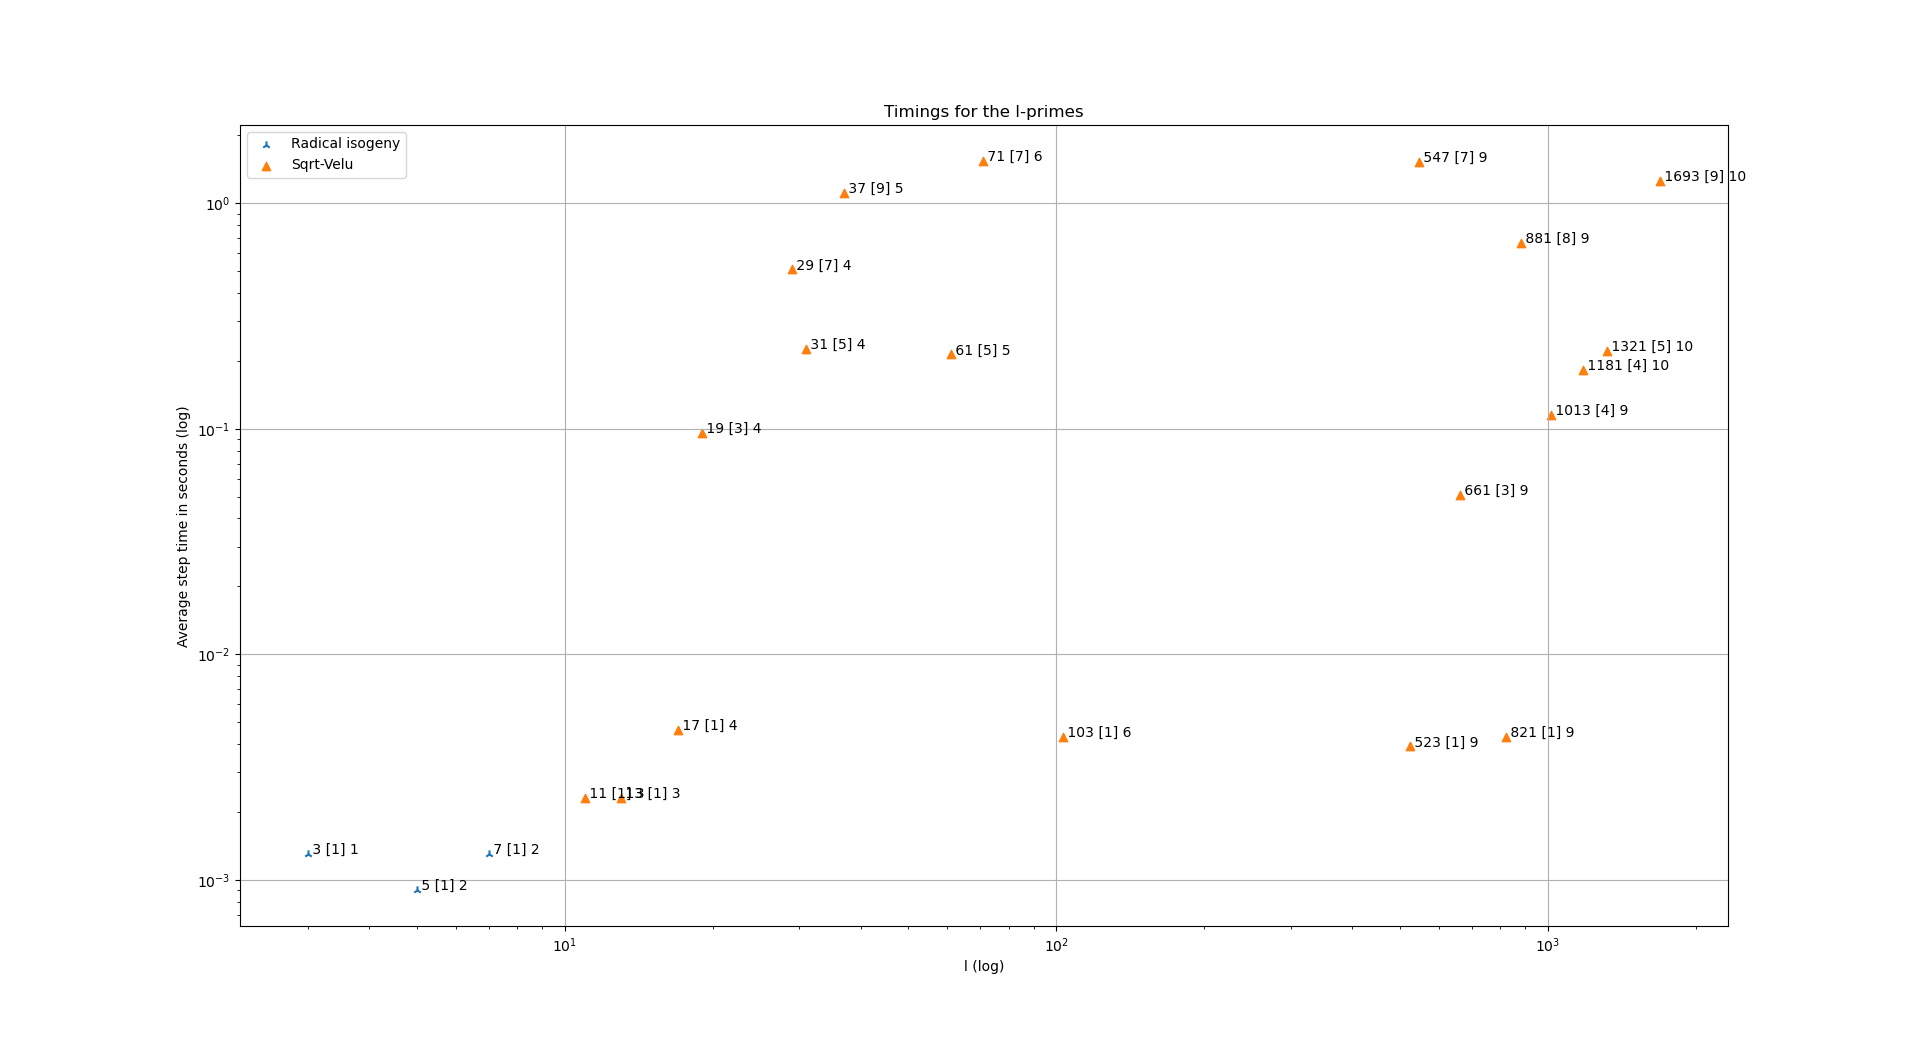
\includegraphics[scale=0.38]{timings}
	\caption{Timing, degree and $\log_2$ for $l$-primes}
\end{figure}
\end{center}
Finally we should mention the code has been ran through \textit{Valgrind} with the \textit{--leak-check} parameter set to \textit{yes} to check for memory leakage.
No such leakage is reported and the code is memory-safe.
We also used \textit{gprof} to get a better look at the inner timings of each functions.
For the complete (with very low bounds) exchange available in \texttt{example/}, the three functions that used the most processing time were
\newcommand{\functi}[1]{\texttt{\detokenize{#1}}}
\begin{enumerate}
	\item \functi{MG_xADD} with 1352762 calls.
	\item \functi{MG_xDBL_const} with 1341432 calls.
	\item \functi{MG_point_init} with 26130 calls.
\end{enumerate}
The first two were used in \functi{MG_ladder_iter_} which had an average of $17$ micro-seconds per call (2282 calls).
That last function gives a sense of how many points were needed to perform the exchange.
This is also the realization that our structure may have been too rigid.
Passing only the $x$-coordinate when manipulating points and making sure all points are  normalized at all time could have been a faster option.






\end{document}
